\documentclass[english]{article}

\usepackage[latin9]{inputenc}
\usepackage[letterpaper]{geometry}
\geometry{verbose,tmargin=1in,bmargin=1in,lmargin=1in,rmargin=1in}
\usepackage{graphicx}
\usepackage{amsmath}
\usepackage{amssymb}
\usepackage{listings}
\usepackage{tikz}
\usetikzlibrary{arrows}
%\usetikzlibrary{graphdrawing}
%\usetikzlibrary{graphs}
%\usegdlibrary{trees}

\title{ESE 605 Homework 3}
\author{Stephen Phillips}
\date{\today }


\begin{document}
\maketitle
\subsection*{Problem 1}
What does the code \textit{incr(i,i)} do on a pass by reference argument? On a pass by copy/restore?

If the pseudo-code is as follows:
\begin{lstlisting}
 function incr(reference i, reference j):
  i = i + 1;
  j = j + 1;
 end function
\end{lstlisting}

Then a pass by reference for \textit{incr(i,i)} would increment \textit{i} twice. %Not sure of the following sentence ....
On pass by copy/restore it should do the same. The reference given to the function will be the same for both \textit{i} and \textit{j} so it will increment twice


\subsection*{Problem 2}
The dependency graph of the processes is as follows:
\begin{figure}[h!]
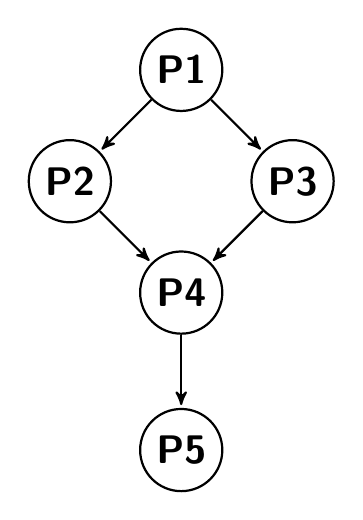
\begin{tikzpicture}[->,>=stealth',shorten >=1pt,auto,node distance=2cm,
  thick,main node/.style={circle,draw,font=\sffamily\Large\bfseries}]

  \node[main node] (1) {P1};
  \node[main node] (2) [below left of=1] {P2};
  \node[main node] (3) [below right of=1] {P3};
  \node[main node] (4) [below right of=2] {P4};
  \node[main node] (5) [below of=4] {P5};

  \path[every node/.style={font=\sffamily\small}]
    (1) edge node { } (2)
        edge node { } (3)
    (2) edge node { } (4)
    (3) edge node { } (4)
    (4) edge node { } (5);
\end{tikzpicture}
\end{figure}

So we run the following code:
\begin{table}[h!]
\begin{tabular}{|c|c|c|}
\hline
\textbf{Initialize Semaphores} & \textbf{Process 1} & \textbf{Process 2}  \\

\begin{lstlisting}
S1.initialize(0)
S2.initialize(0)
S3.initialize(0)
\end{lstlisting}
 & 
 \begin{lstlisting}
// Process 1 code ...
V(S1)
V(S1)
\end{lstlisting}
& 
\begin{lstlisting}
P(S1)
// Process 2 code ...
V(S2)
\end{lstlisting} \\ \hline \hline
\textbf{Process 3} & \textbf{Process 4} & \textbf{Process 5} \\

\begin{lstlisting}
P(S1)
// Process 3 code ...
V(S2)
\end{lstlisting}
& 
\begin{lstlisting}
P(S2)
P(S2)
// Process 4 code ...
V(S3)
\end{lstlisting}
&
\begin{lstlisting}
P(S3)
// Process 5 code ...
\end{lstlisting} \\\hline


\end{tabular}
\end{table}


\subsection*{Problem 3}
The dependency graph of the processes is as follows:

\begin{figure}[h!]
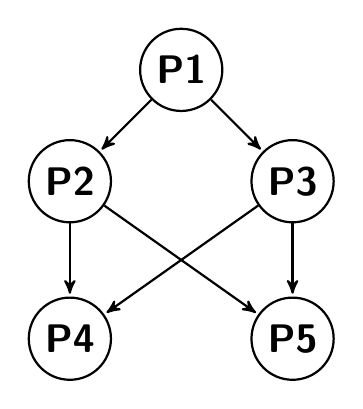
\begin{tikzpicture}[->,>=stealth',shorten >=1pt,auto,node distance=2cm,
  thick,main node/.style={circle,draw,font=\sffamily\Large\bfseries}]

  \node[main node] (1) {P1};
  \node[main node] (2) [below left of=1] {P2};
  \node[main node] (3) [below right of=1] {P3};
  \node[main node] (4) [below of=2] {P4};
  \node[main node] (5) [below of=3] {P5};

  \path[every node/.style={font=\sffamily\small}]
    (1) edge node { } (2)
        edge node { } (3)
    (2) edge node { } (4)
        edge node { } (5)
    (3) edge node { } (4)
        edge node { } (5);
\end{tikzpicture}
\end{figure}

\subsubsection*{Part a}
Here we are allowed to only use binary semaphores. So we do the following:
\begin{table}[ht!]
\begin{tabular}{|c|c|c|}
\hline
\textbf{Initialize Semaphores} & \textbf{Process 1} & \textbf{Process 2}  \\

\begin{lstlisting}
S1.initialize(0)
S2.initialize(0)
S3.initialize(0)
\end{lstlisting}
 & 
 \begin{lstlisting}
// Process 1 code ...
V(S1)
\end{lstlisting}
& 
\begin{lstlisting}
P(S1)
// Process 2 code ...
V(S1) // For P3
V(S2)
\end{lstlisting} \\ \hline \hline
\textbf{Process 3} & \textbf{Process 4} & \textbf{Process 5} \\

\begin{lstlisting}
P(S1)
// Process 3 code ...
V(S1) // For P2
V(S3)
\end{lstlisting}
& 
\begin{lstlisting}
P(S2)
P(S3)
// Process 4 code ...
V(S1)
V(S3) // For P5
\end{lstlisting}
&
\begin{lstlisting}
P(S2)
P(S3)
// Process 5 code ...
V(S1)
V(S3) // For P4
\end{lstlisting} \\\hline

\end{tabular}
\end{table}

\subsubsection*{Part b}
Here we are allowed to use general counting semaphores. So we do the following:
\begin{table}[ht!]
\begin{tabular}{|c|c|c|}
\hline
\textbf{Initialize Semaphores} & \textbf{Process 1} & \textbf{Process 2}  \\

\begin{lstlisting}
S1.initialize(0)
S2.initialize(0)
S3.initialize(0)
\end{lstlisting}
 & 
 \begin{lstlisting}
// Process 1 code ...
V(S1)
V(S1)
\end{lstlisting}
& 
\begin{lstlisting}
P(S1)
// Process 2 code ...
V(S2)
V(S2)
\end{lstlisting} \\ \hline \hline
\textbf{Process 3} & \textbf{Process 4} & \textbf{Process 5} \\

\begin{lstlisting}
P(S1)
// Process 3 code ...
V(S3)
V(S3)
\end{lstlisting}
& 
\begin{lstlisting}
P(S2)
P(S3)
// Process 4 code ...
\end{lstlisting}
&
\begin{lstlisting}
P(S2)
P(S3)
// Process 5 code ...
\end{lstlisting} \\\hline

\end{tabular}
\end{table}



\subsection*{Problem 4}
\subsubsection*{Part a}
Why do dead locks occur in the dining philosophers problem? Because we have shared resources that must be used exclusively by 1 party/philosopher.
More specifically if we have a situation like this:

\begin{figure}[h!]
 \centering 
 
\includegraphics[scale=0.35]{dining-philosophers-problem-small.jpg}
 \caption{(I'm more partial to the chopsticks myself...)}
\end{figure}


Then if all the philosophers grab the left for at the same time, then need to grab the right fork, they will have to wait until one of the other ones drop it.
If none of the others ever drop it, then they will wait forever and starve. This is the deadlock.

\subsubsection*{Part b}
To fix this problem we will make the philosophers drop the forks after a certain amount of time. We use notation similar to the one used in lecture. Basically
we use a simple solution: Give an ordering to the forks. 

\begin{figure}[h!]
\begin{lstlisting}
var fork: array[0..4] of semaphores=1
philosopher i
repeat
  first = min( i, i+1 mod 5 )
  next = max( i, i+1 mod 5 )
  wait( first )
  wait( next )
  ...
  eat
  ...
  post( first );
  post( next );
  ...
  think
  ...
forever
 
 \end{lstlisting}
 
 This prevents deadlock by not allowing everyone to pick up the left fork at the same time. Suppose this did not prevent deadlock, then there must be some fork, say \textit{i} 
 that is locked forever. Then the philosopher using that must be waiting for a fork, \textit{j}, which must be great than \textit{i}. Keep going along the chain and eventually
 you must, since this is deadlocked, get back to \textit{i}, which means \textit{i} $>$ \textit{i}, which is nonsense. So we must have that this prevents deadlock. This is not very
 efficient, and there are more efficient solutions but this is the simplest (in my mind) that prevents deadlock. 
 
\end{figure}


\end{document}